\chapter{Diseños individuales para la iteración competitiva de Johan Sebastian Salvatierra Gutierrez}
\label{ape:disenyoJohan}

En este apéndice se muestran los diseños individuales realizados por Johan Sebastian Salvatierra Gutierrez para la iteración competitiva. En primer lugar, la Figura \ref{Johan1} donde se puede ver a la izquierda un panel que permite subir un documento, en concreto PDF, en la derecha se encuentra el editor y arriba está el encabezado con un menú para acceder a las demás pantallas y un botón de ajustes para configurar la pantalla de inicio. En segundo lugar tenemos la Figura \ref{Johan2} donde se encuentra la anterior pantalla pero con todas los ajustes disponibles. En este caso en el lado izquierdo se encuentra dos paneles el panel de arriba es para insertar un documento y el panel de abajo es donde se dispondrá de funciones para la creación de ejercicios. En tercer lugar la Figura \ref{Johan3} muestra qué pasa si se selecciona el menú de navegación. En cuarto lugar, la Figura \ref{Johan4} donde se muestra la pantalla de ``Ayuda'' donde aparecerán diferentes videos para entender el funcionamiento de la aplicación web. En quinto lugar, está la Figura \ref{Johan5} donde se nos mostrara en formato carta información sobre los integrantes que crearon esta aplicación. Por último, tenemos figuras relacionas con los distintos ejercicios que se proporcionan.

\begin{figure}[ht!]
  \centering
  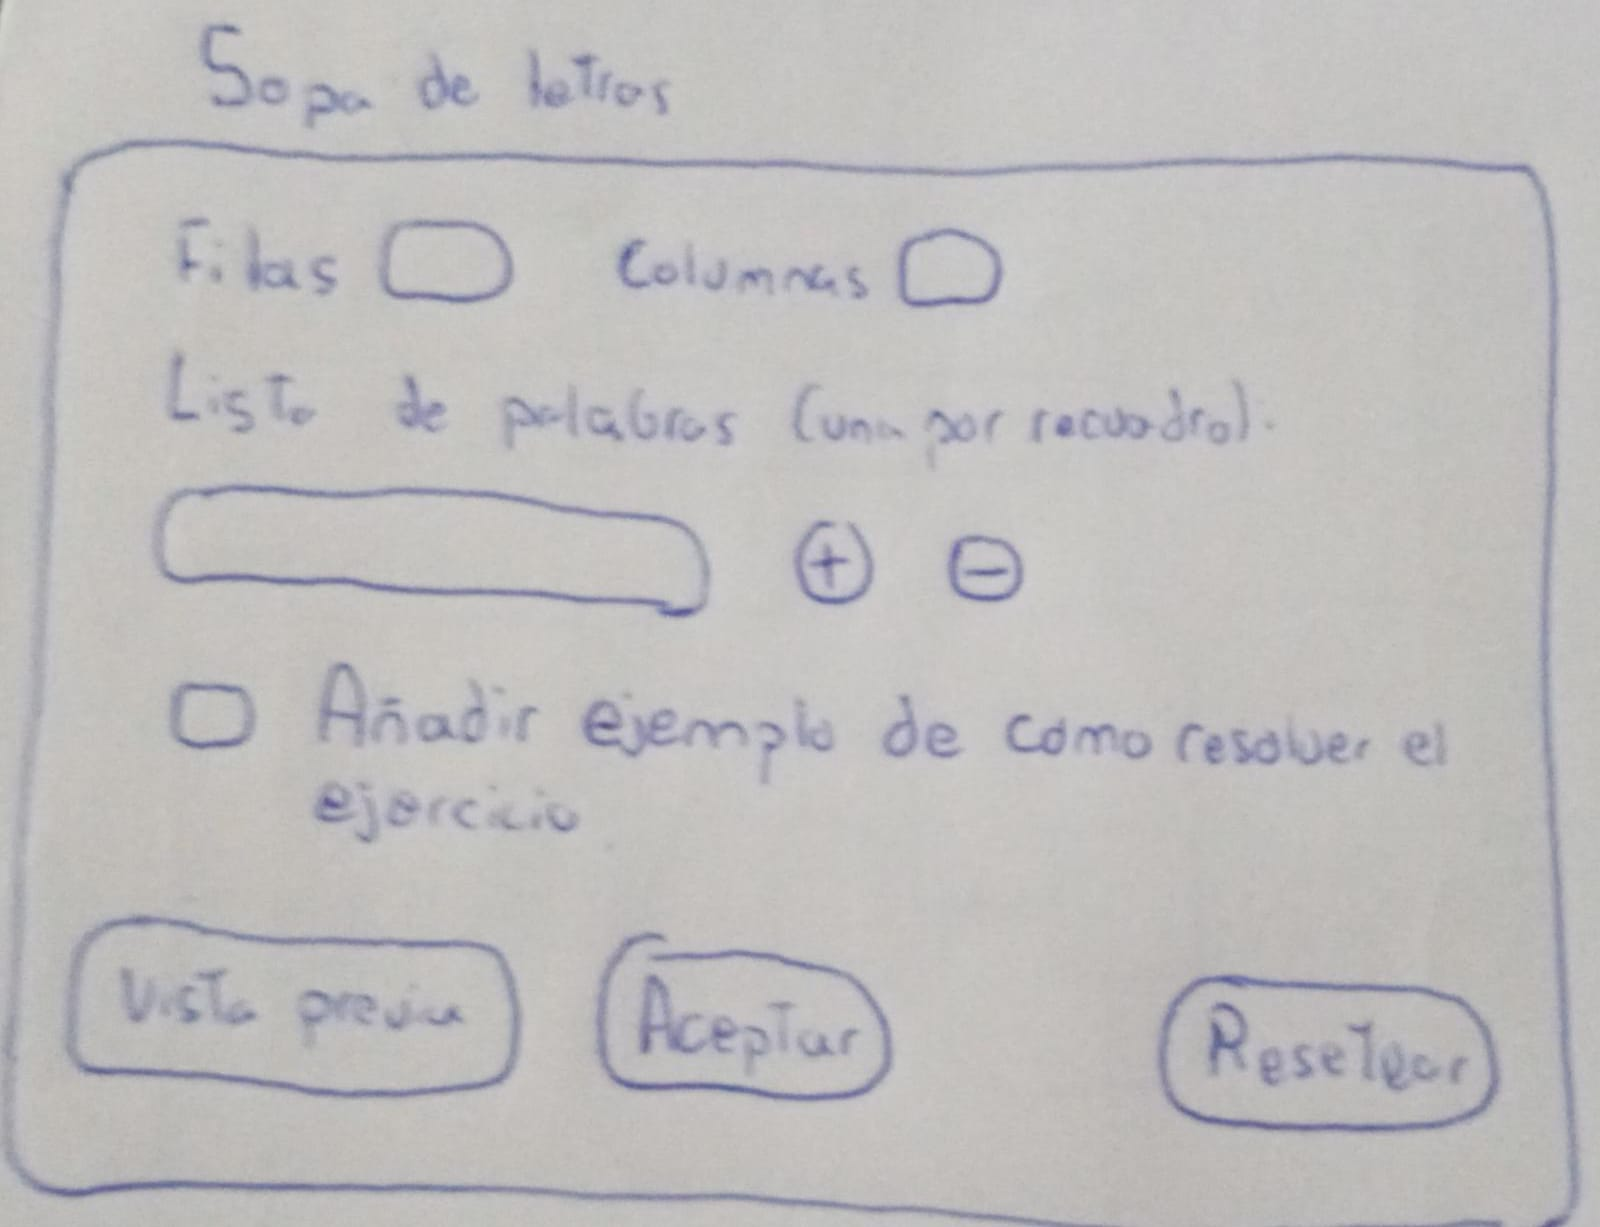
\includegraphics[width=0.6\textwidth]{Diseño/Johan/Johan1.jpeg}
  \caption{Diseño pantalla de inicio de Johan.}
  \label{Johan1}
\end{figure}

\begin{figure}[ht!]
  \centering
  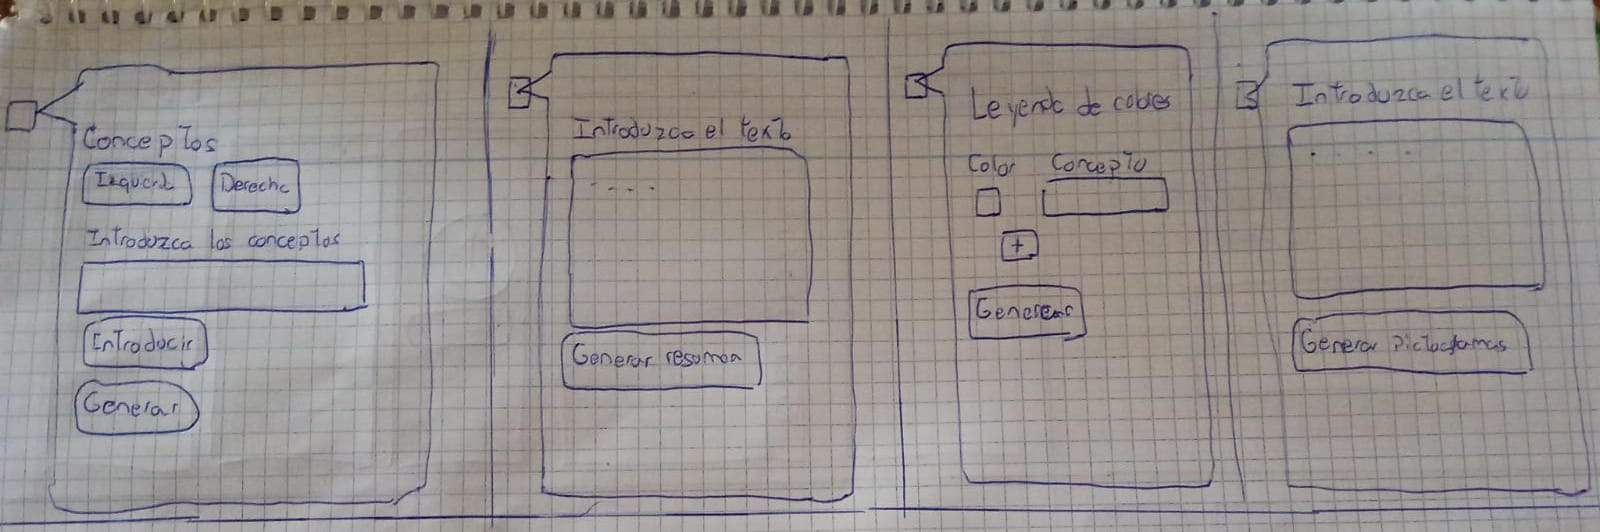
\includegraphics[width=0.6\textwidth]{Diseño/Johan/Johan2.jpeg}
  \caption{Diseño pantalla de inicio completa de Johan.}
  \label{Johan2}
\end{figure}

\begin{figure}[ht!]
  \centering
  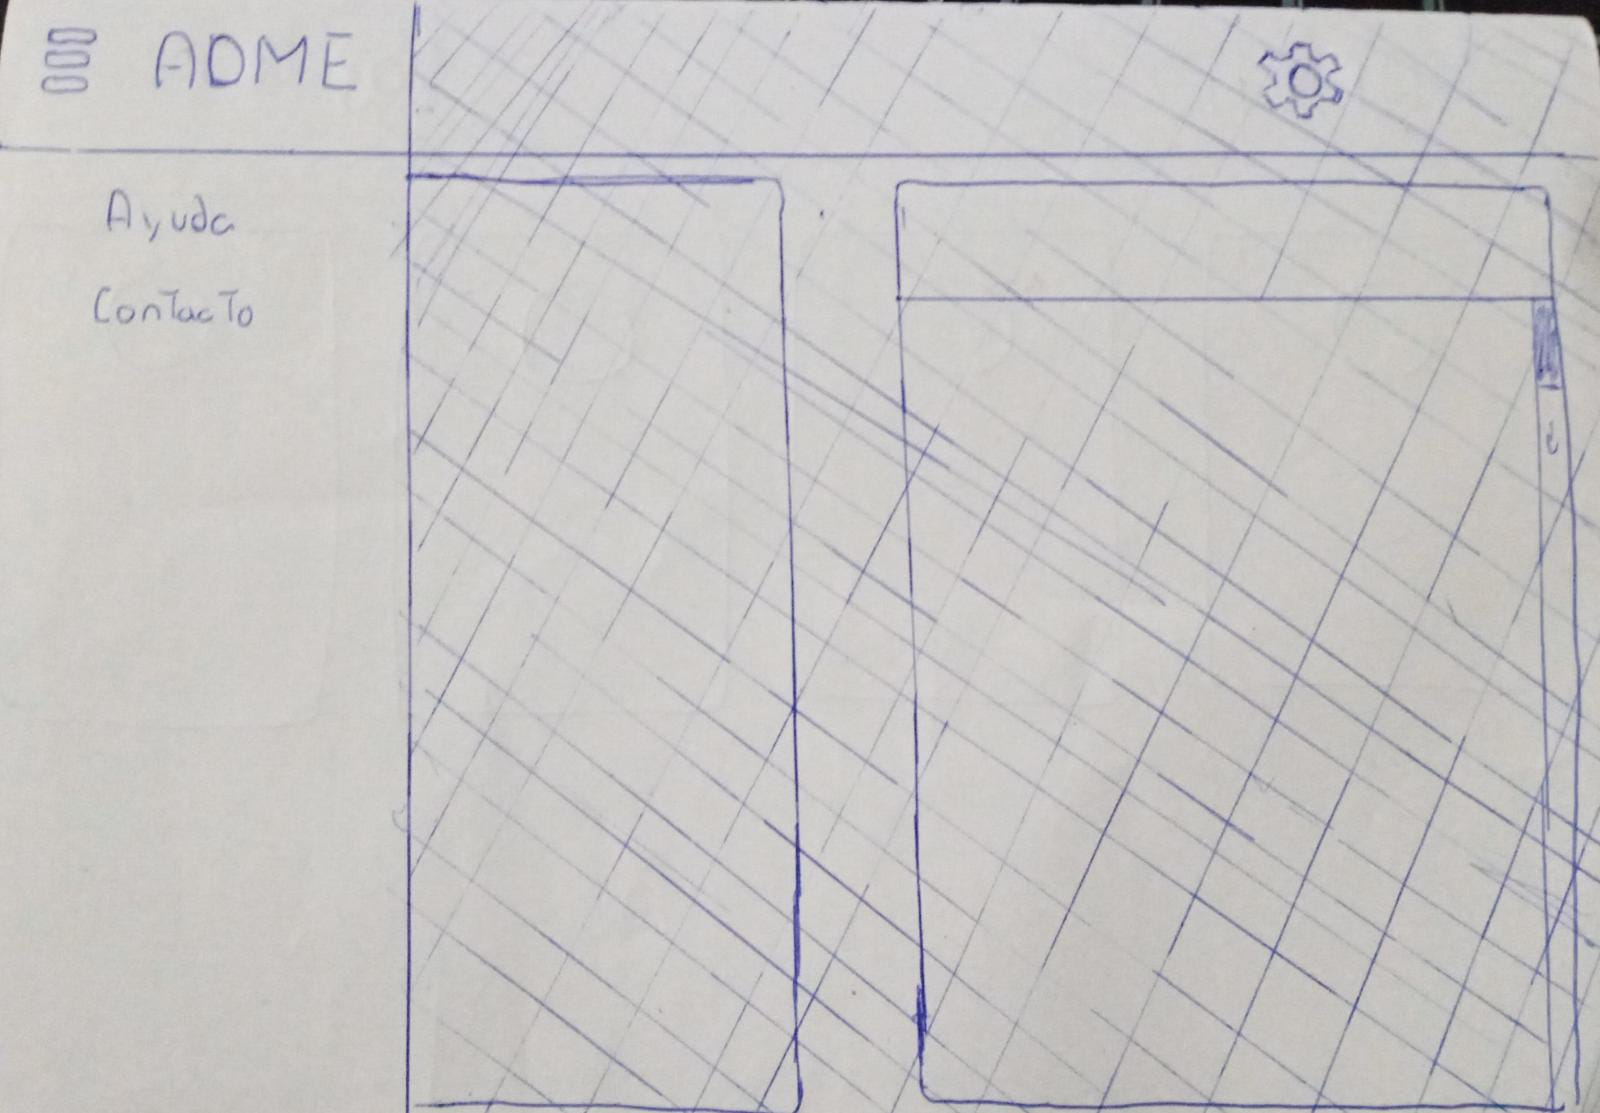
\includegraphics[width=0.6\textwidth]{Diseño/Johan/Johan3.jpeg}
  \caption{Diseño de barra de navegación de Johan.}
  \label{Johan3}
\end{figure}

\begin{figure}[ht!]
  \centering
  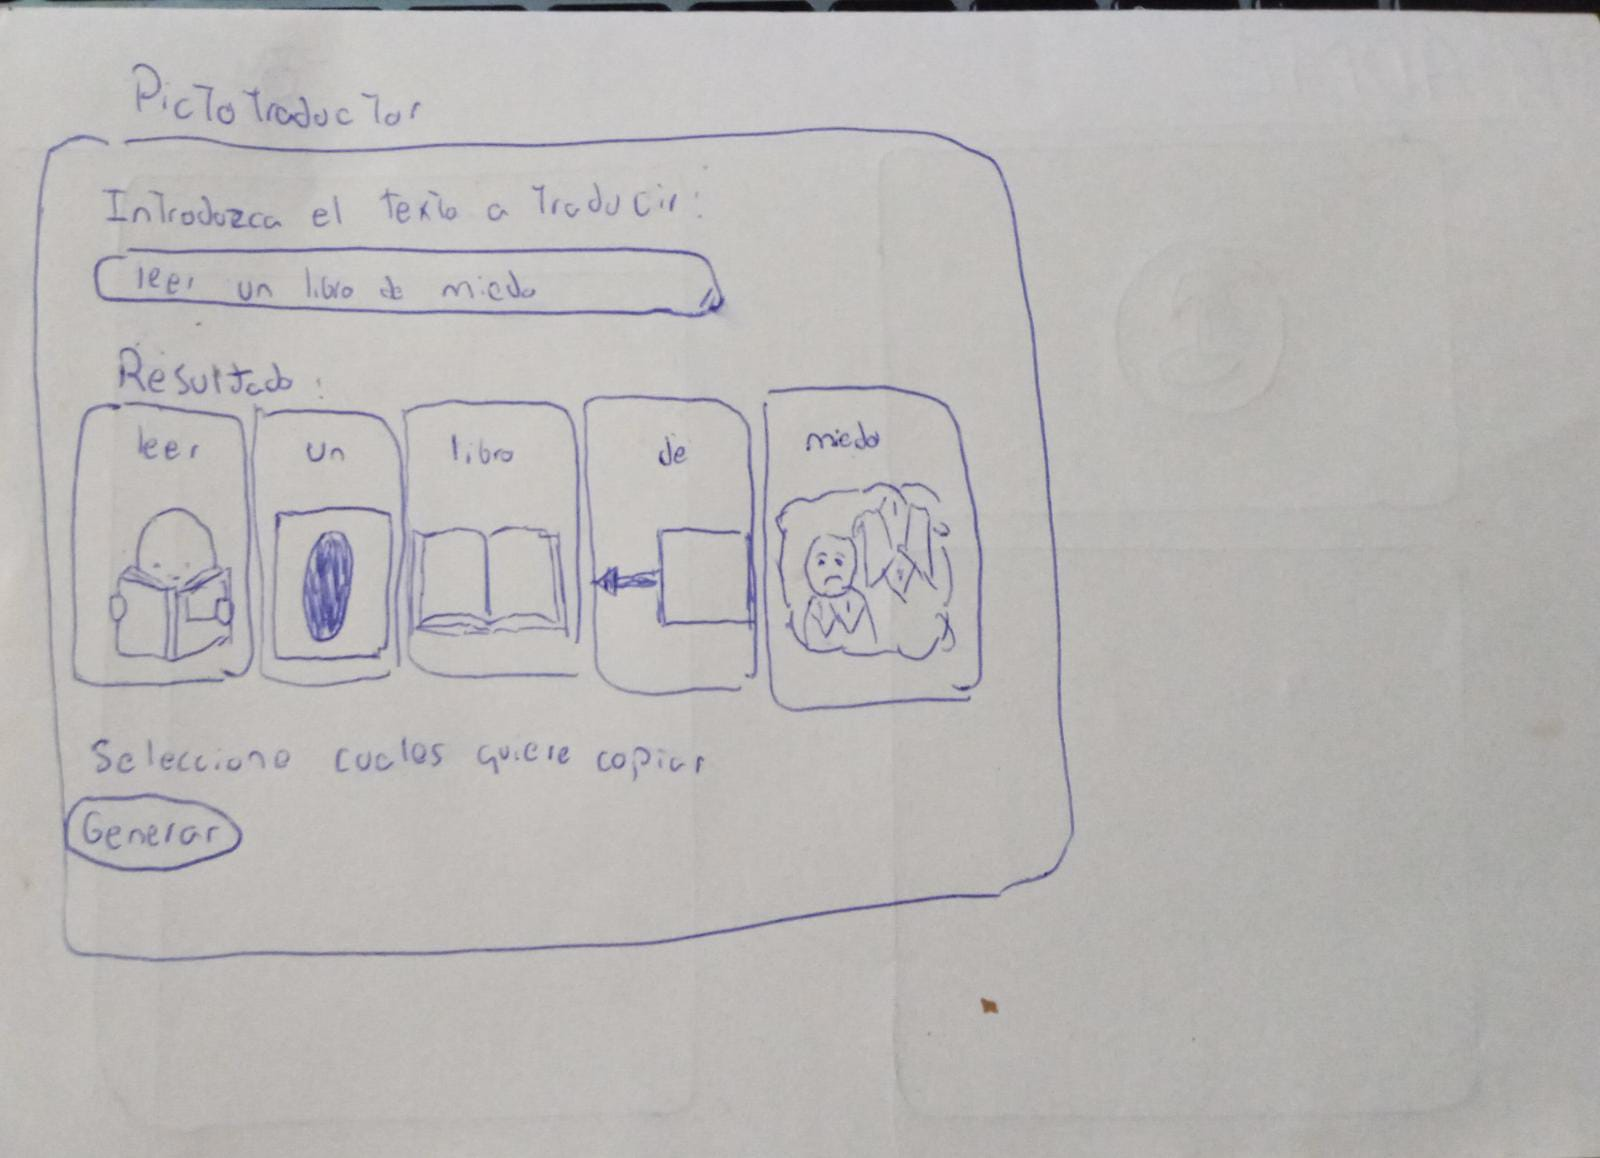
\includegraphics[width=0.6\textwidth]{Diseño/Johan/Johan4.jpeg}
  \caption{Diseño de página de información de Johan.}
  \label{Johan4}
\end{figure}

\begin{figure}[ht!]
  \centering
  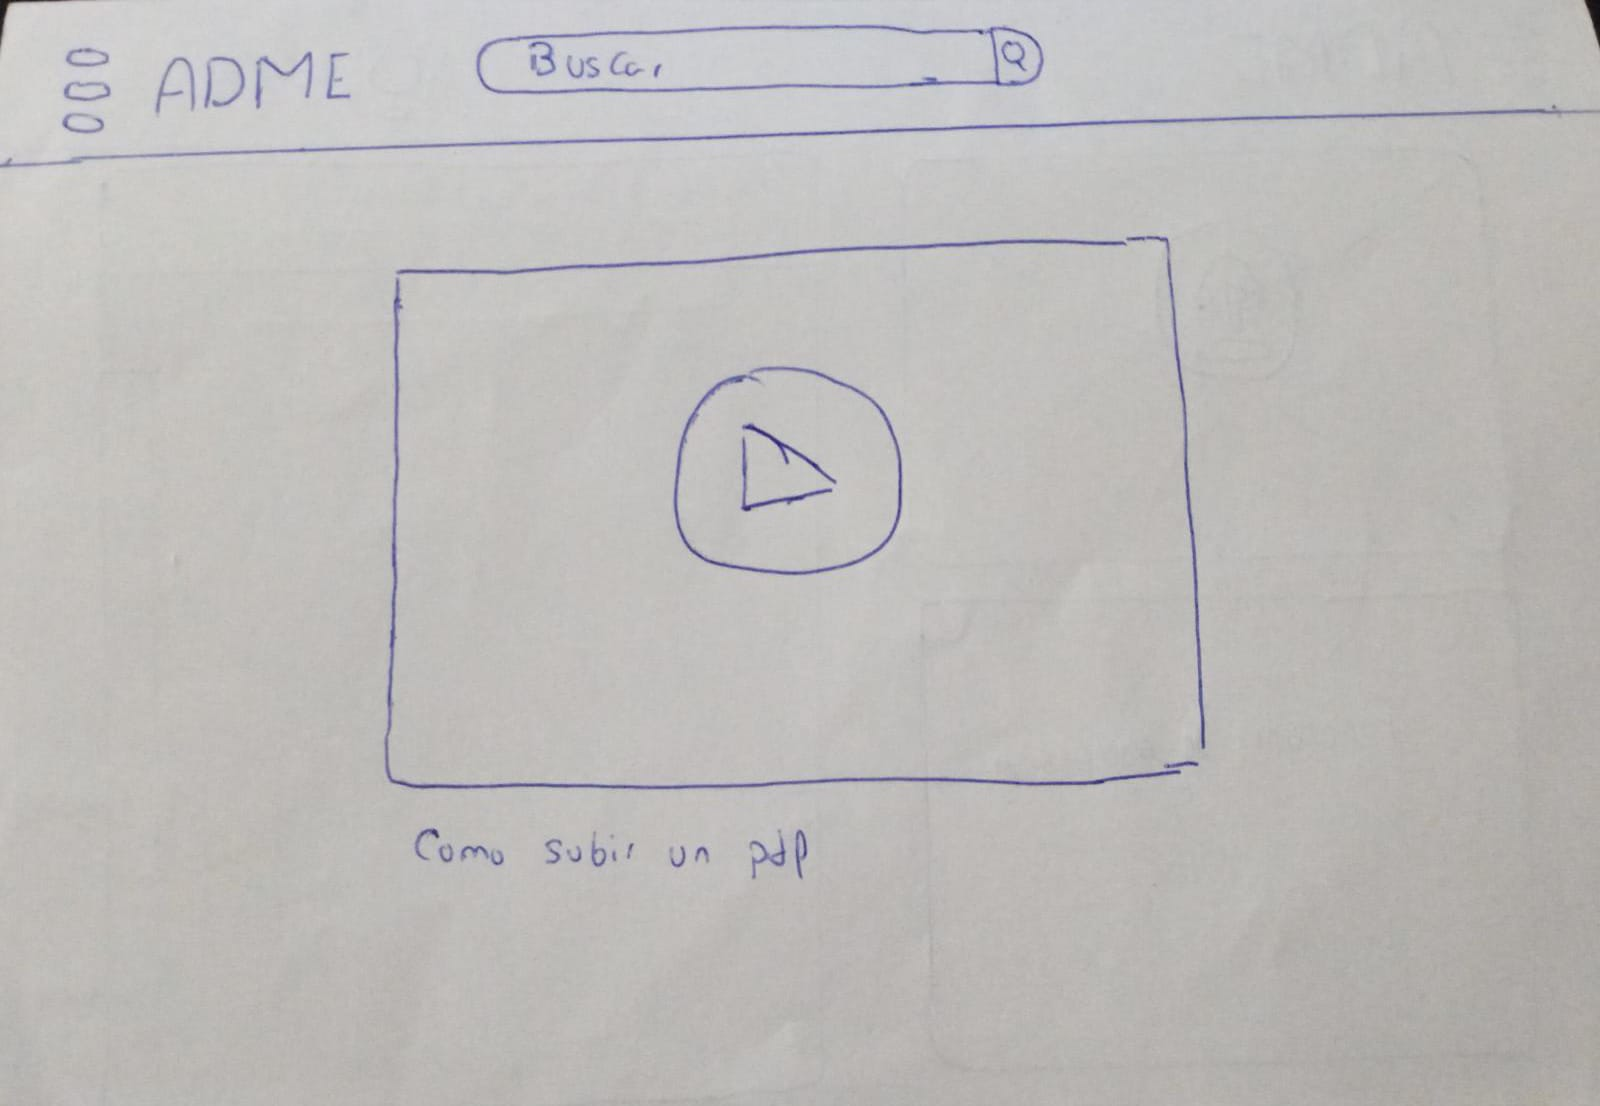
\includegraphics[width=0.6\textwidth]{Diseño/Johan/Johan5.jpeg}
  \caption{Diseño de página de sobre nosotros de Johan.}
  \label{Johan5}
\end{figure}

\begin{figure}[ht!]
  \centering
  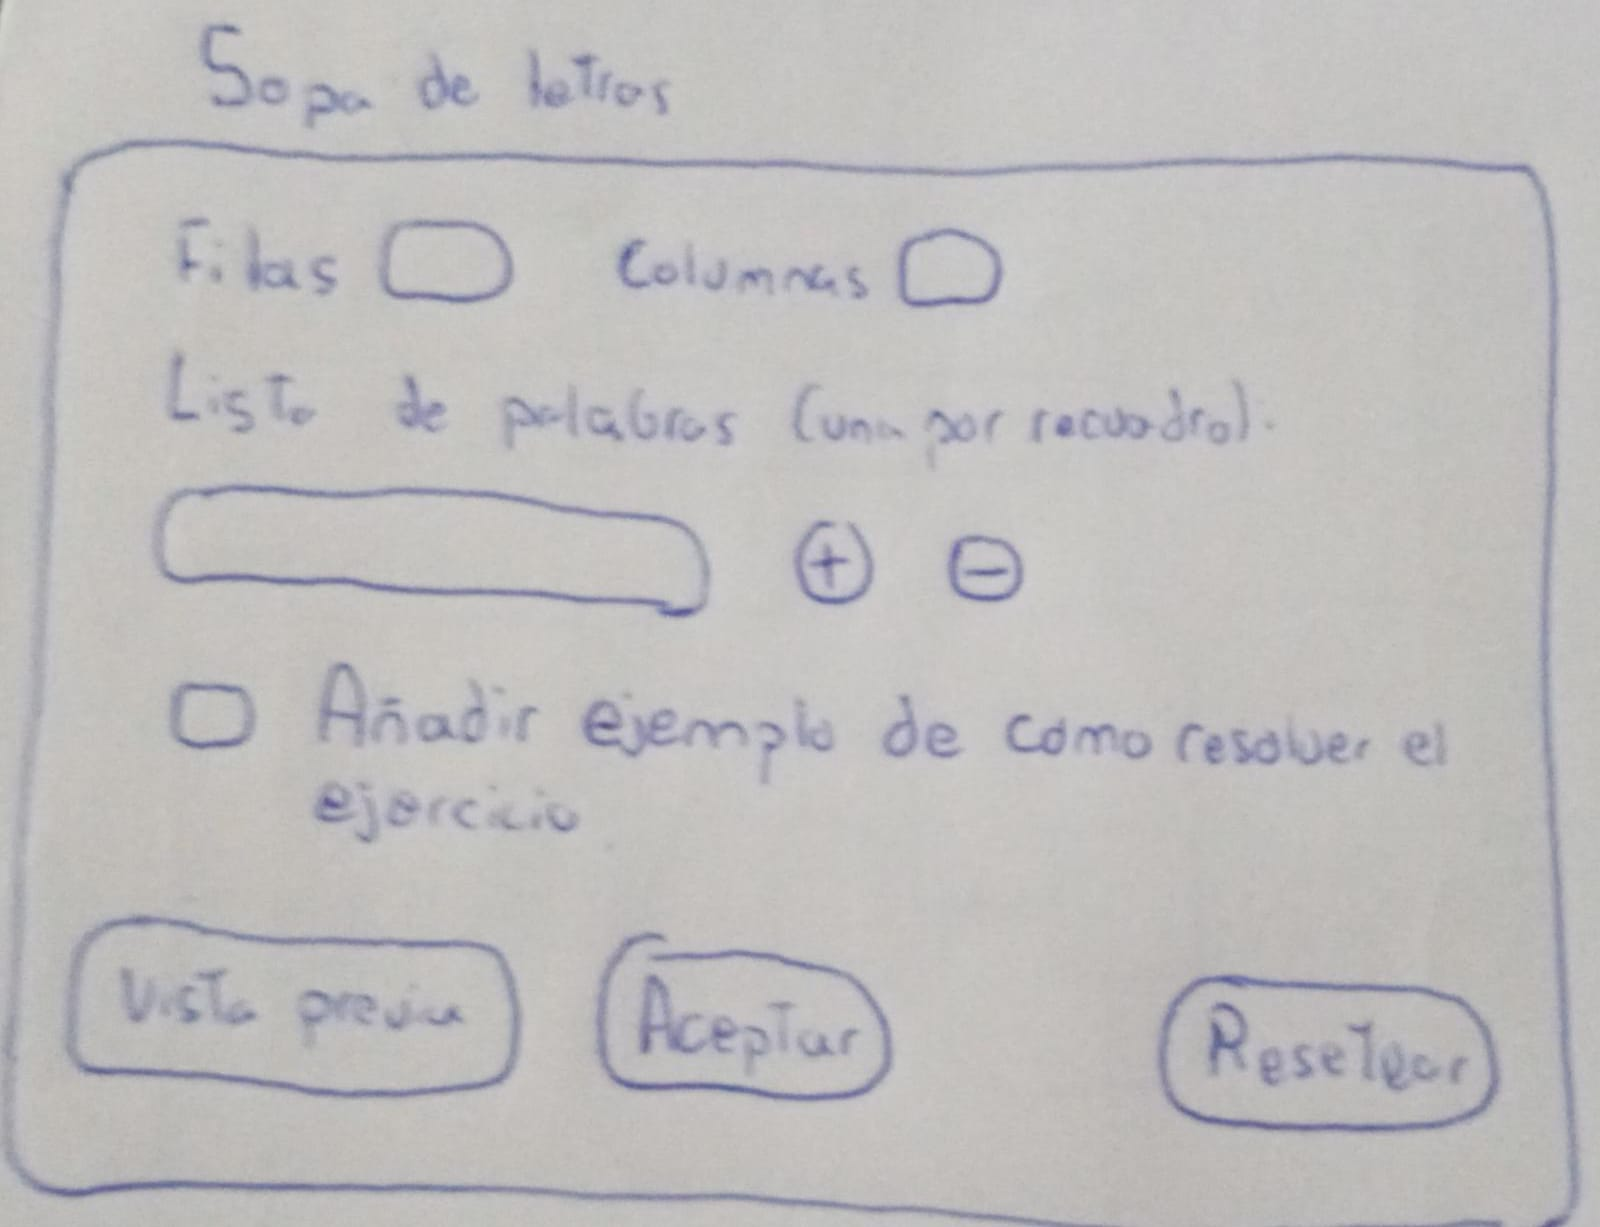
\includegraphics[width=0.6\textwidth]{Diseño/Johan/Johan6}
  \caption{Diseño de sopa de letras.}
  \label{Johan6}
\end{figure}

\begin{figure}[ht!]
  \centering
  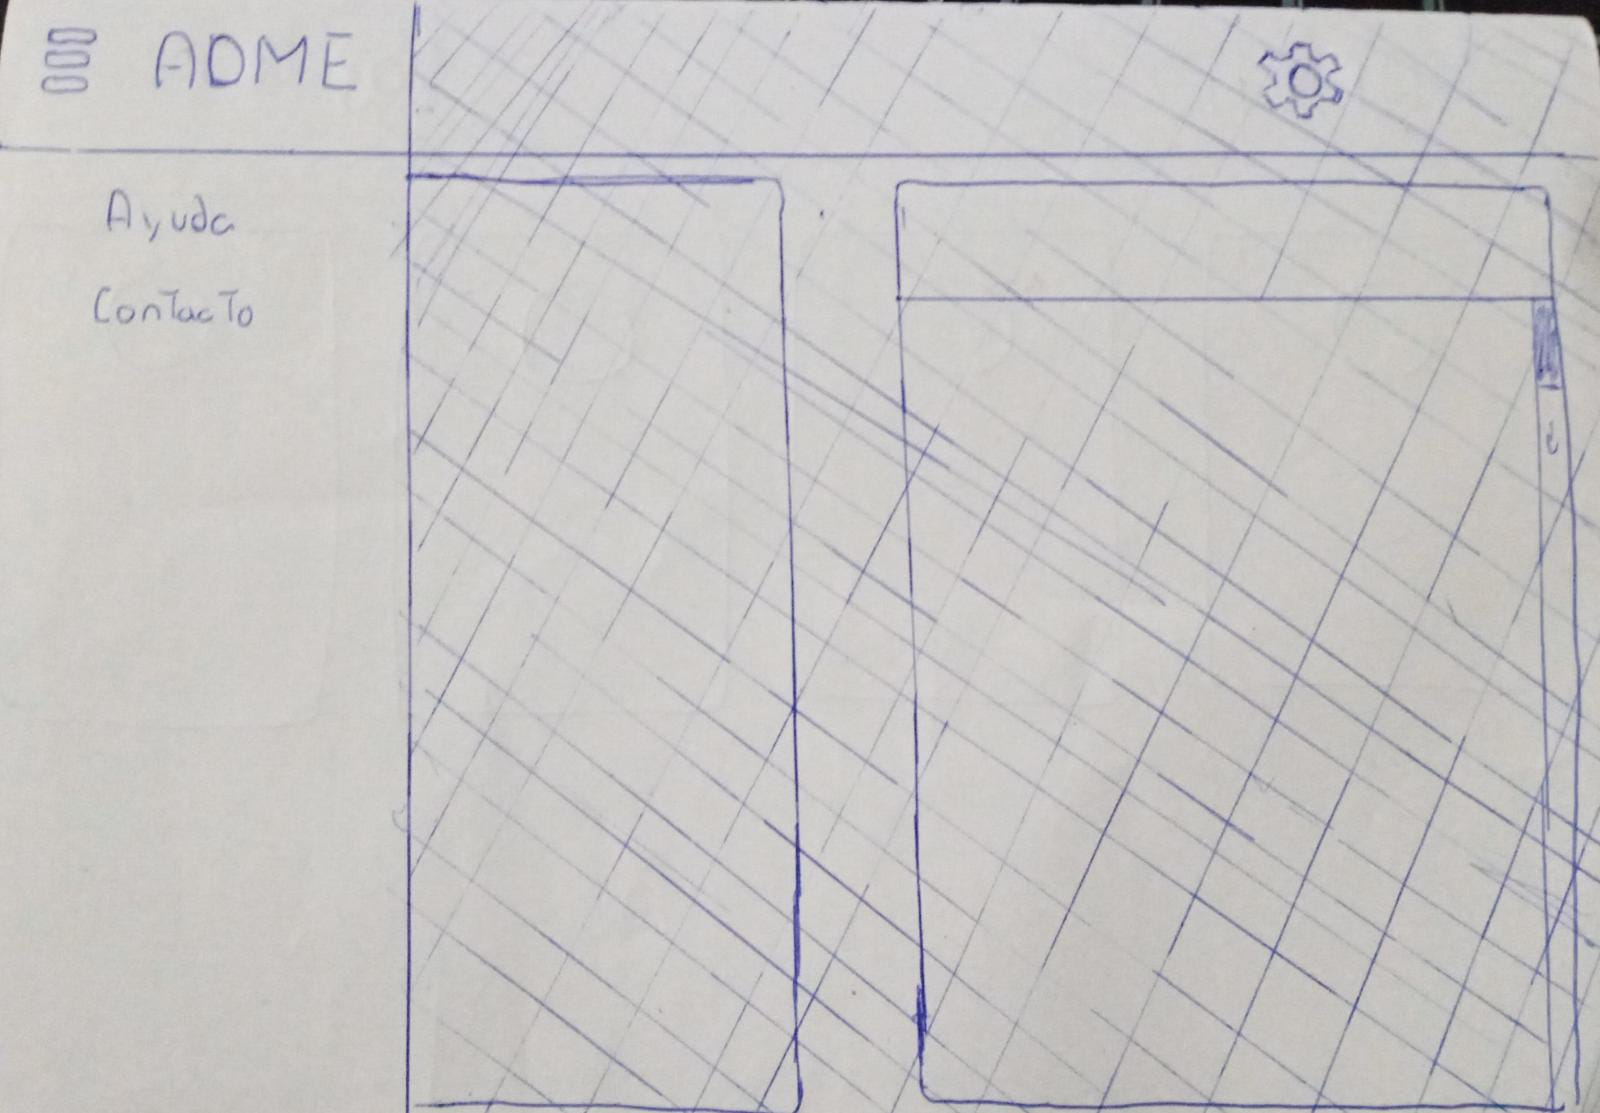
\includegraphics[width=0.6\textwidth]{Diseño/Johan/Johan7.jpeg}
  \caption{Diseño de ejercicios de flechas de Johan.}
  \label{Johan7}
\end{figure}

\begin{figure}[ht!]
  \centering
  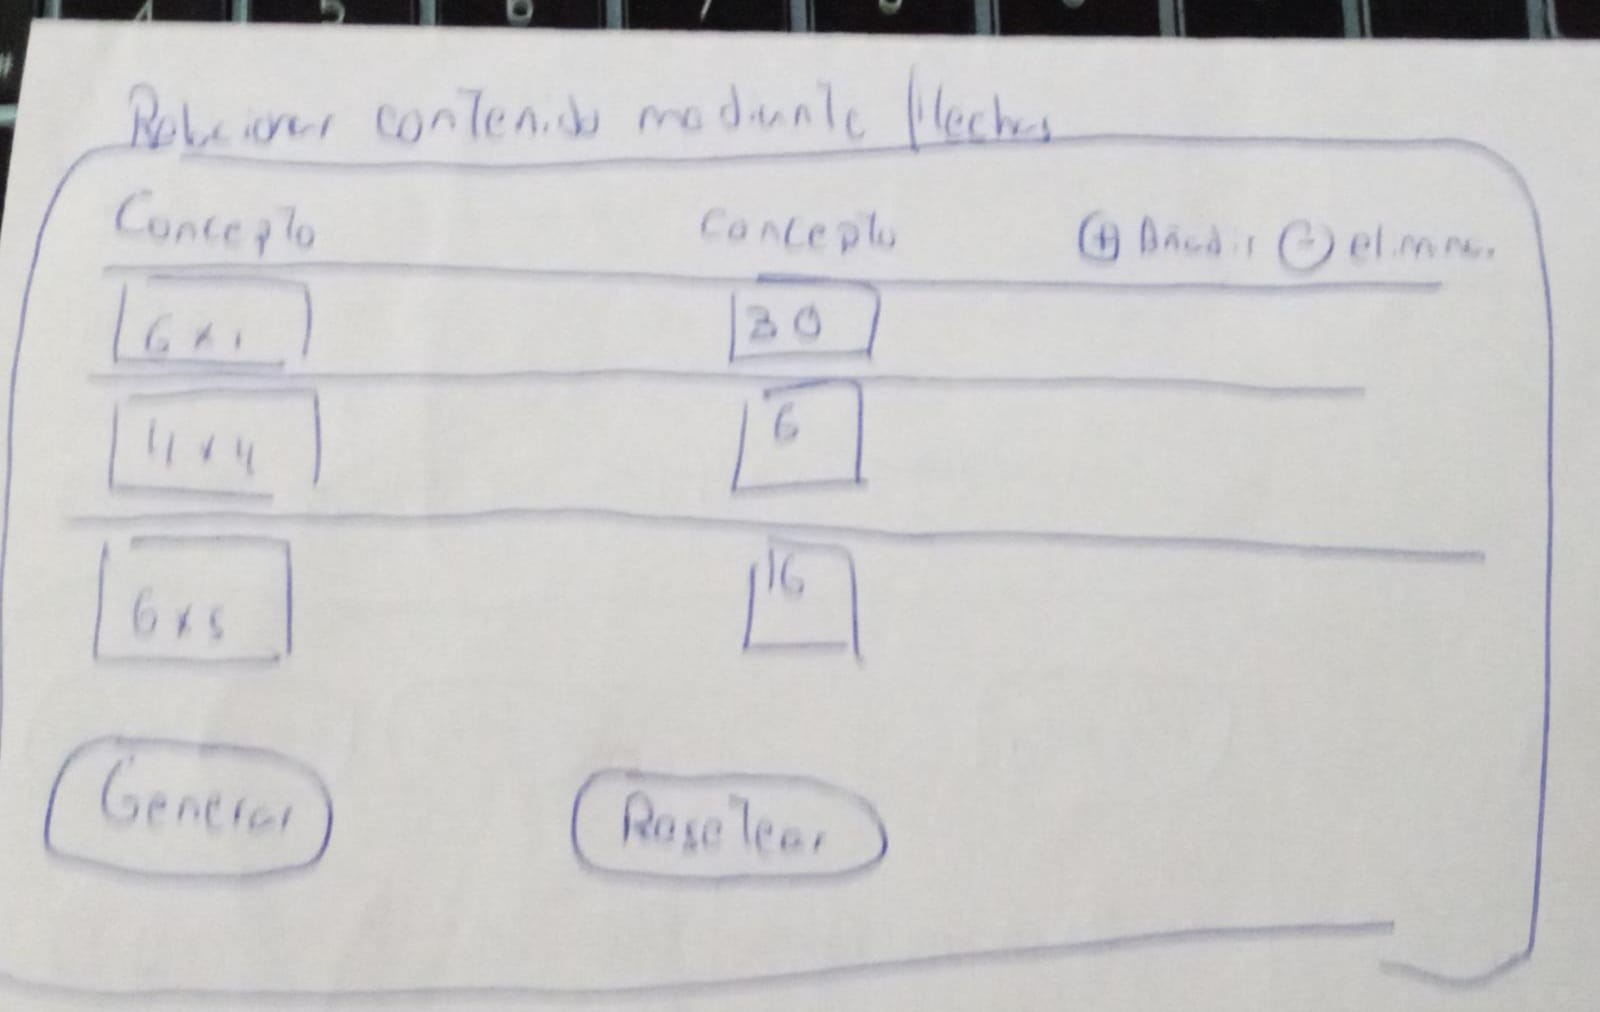
\includegraphics[width=0.6\textwidth]{Diseño/Johan/Johan8.jpeg}
  \caption{Diseño de leyenda de Johan.}
  \label{Johan8}
\end{figure}

\begin{figure}[ht!]
  \centering
  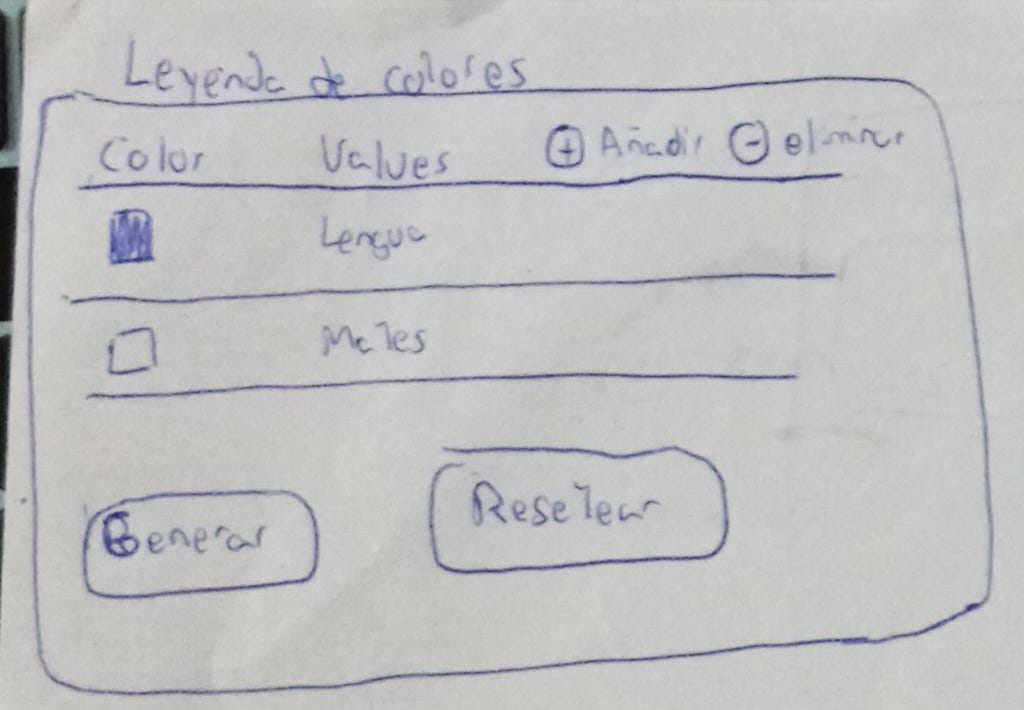
\includegraphics[width=0.6\textwidth]{Diseño/Johan/Johan9.jpeg}
  \caption{Diseño de leyenda de Johan.}
  \label{Johan9}
\end{figure}